\section{Supervised learning}


\frame{\frametitle{The machine learning triad}
\begin{figure}
	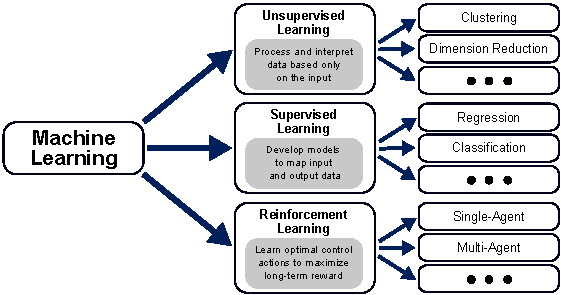
\includegraphics[width=11cm]{fig/lec01/Machine_Learning_Disciplines.pdf}
	\caption{Disciplines of machine learning 
	}
	\label{fig:Machine_Learning_Disciplines_2}
\end{figure}
}

\frame{\frametitle{Introductory material}
Machine learning (ML) and especially the field of supervised learning (SL) is extensively researched and taught.
\begin{itemize}
	\item Renowned online courses
	\begin{itemize}
		\item \href{https://de.coursera.org/learn/machine-learning}{\textit{Coursera ML} by Stanford's Andrew Ng}
		\item \href{https://www.fast.ai/}{\textit{Practical deep learning for coders} by fast.ai}
		\item \href{https://www.kaggle.com/learn/overview}{\textit{Intro to ML} by Kaggle Courses}
	\end{itemize}\pause
	\item Books classics
	\begin{itemize}
		\item \href{http://users.isr.ist.utl.pt/~wurmd/Livros/school/Bishop\%20-\%20Pattern\%20Recognition\%20And\%20Machine\%20Learning\%20-\%20Springer\%20\%202006.pdf}{\textit{Pattern Recognition and Machine Learning} by C. M. Bishop}
		\item \href{http://www-stat.stanford.edu/~tibs/ElemStatLearn/printings/ESLII_print10.pdf}{\textit{The Elements of Statistical Learning} by Hastie et al.}
		\item \href{https://www.deeplearningbook.org/}{\textit{Deep Learning} by I. Goodfellow, Y. Bengio, and A. Courville}
	\end{itemize}
\end{itemize}
}


%  ML hype in industry
\frame{\frametitle{Machine learning in industry}
	Machine learning applications are a \href{https://magazine.startus.cc/how-machine-learning-is-changing-the-major-industries/}{fast growing industry itself}, and enhance more and more automation in classical industry as well.
	
	Among others, popular industries are:
	\begin{itemize}
		\item Embedded systems,
		\item Mobility, and
		\item Digital assistants
	\end{itemize}
	
	Most applications are of the supervised type.
	
	The demand for highly skilled ML engineers is growing correspondingly.
}

\frame{\frametitle{Instances of ML applications}
	\begin{itemize}
		\item Recommendation systems
		\begin{itemize}
			\item Which ads to display on a website?
			\item Which items are \href{https://tech.instacart.com/deep-learning-with-emojis-not-math-660ba1ad6cdc}{most likely put into cart next} by the user?
		\end{itemize}\pause
		\item Forecasting
		\begin{itemize}
			\item Weather, sales, \href{https://eng.uber.com/forecasting-introduction/}{geospatial Uber calls}, \href{https://www.kaggle.com/c/recruit-restaurant-visitor-forecasting}{restaurant}/\href{https://towardsdatascience.com/web-traffic-forecasting-f6152ca240cb}{website} traffic
			\item Material attrition in engineering processes (predictive maintenance)
		\end{itemize}\pause
		\item Classification/Regression
		\begin{itemize}
			\item Speech assistants (Alexa/Siri), pedestrial detection (autonomous driving), \href{https://www.kaggle.com/c/severstal-steel-defect-detection}{fault detection in engineering processes}
			\item \href{https://openai.com/blog/chatgpt}{large language models (LLM)}, credit scoring (fintech) 
		\end{itemize}\pause
		\item \href{https://stablediffusionweb.com/}{Generative models}

	\end{itemize}
}

%  Kaggle comps
\frame{\frametitle{ML competitions with price pool}
	\begin{figure}
		
\includegraphics[width=9cm]{fig/lec08/comp_logos.pdf}
		\caption{Kaggle and DrivenData}
		\label{fig:comp_logos}
	\end{figure}
	
	Open ML competition platforms like \href{https://www.kaggle.com/}{kaggle} or \href{https://www.drivendata.org/competitions/}{DrivenData} offer a multitude of diverse competitions to participate in at no cost.
	
	\begin{itemize}
		\item Most competitions come with a decent price pool of 15 tsd. dollars up to 1 mil. dollars hosted by stakeholders from the industry and government.
		\item These competitions are almost exclusively of the supervised type, but RL challenges are increasing.
	\end{itemize}
}

%  Typical ML pipeline
\frame{\frametitle{Typical supervised learning pipeline}
	\begin{figure}
		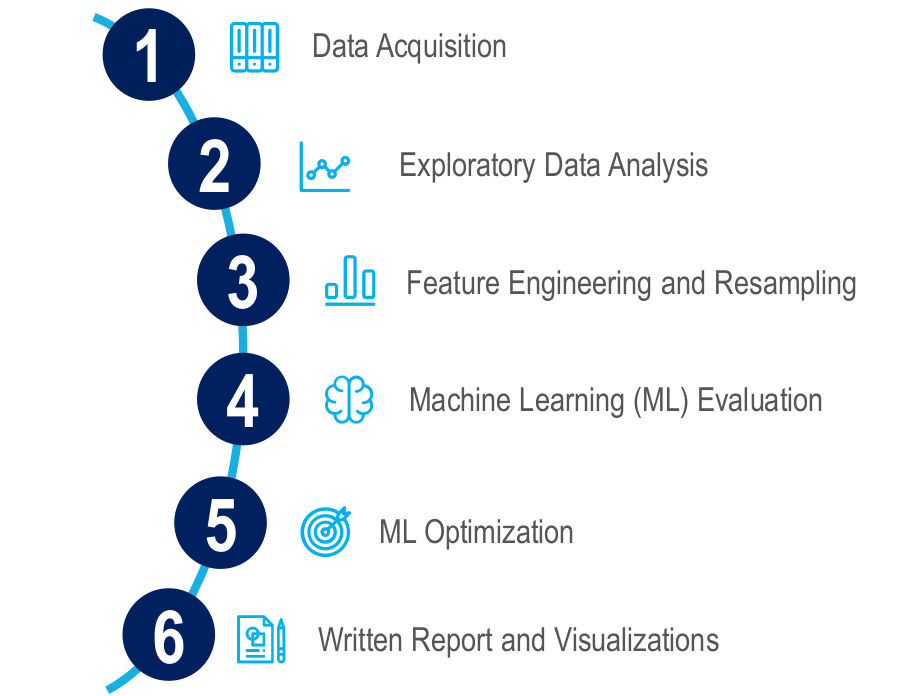
\includegraphics[width=8cm]{fig/lec08/ML_pipeline.png}
		\caption{A typical supervised learning pipeline -- sometimes more art than science}
		\label{fig:ml_pipeline}
	\end{figure}
}


\frame{\frametitle{Supervised learning in reinforcement learning}
	\hl{SL approximates functions, RL approximates policies.} \newline
	
	\pause
	
	However, there are two situations where SL is auxiliary in RL:
	
	\begin{itemize}
		\item Function approximation of (action-)state values, if the number of possible states exceeds any reasonable memory capabability, which is often the case.
		\begin{itemize}
			\item	$v_\pi(x) \approx \hat v(x, \bm w)$ with $\bm w$ being a trainable weight vector.
		\end{itemize} \pause
		\item Imitation learning. A simple-to-implement, deterministic baseline policy is often available, but an RL agent might fail to achieve that performance when learning from scratch. With SL, this baseline policy can be approximated to be the initial behavior of the agent.\pause
		\begin{itemize}
			\item Expert moves in board games.
			\item Basic linear controllers in engineering applications with feedback-loops.
		\end{itemize}
	\end{itemize}
}

%%%%%%%%%%%%%%%%%%%%%%%%%%%%%%%%%%%%%%%%%%%%%%%%%%%%%%%%%%%%%%%%%%
\subsection{Supervised learning problem statement}
%%%%%%%%%%%%%%%%%%%%%%%%%%%%%%%%%%%%%%%%%%%%%%%%%%%%%%%%%%%%%%%%%%

\frame{\frametitle{Supervised learning problem statement}
	\begin{block}{Supervised learning}
		Given a \hl{labeled} data set $\left\langle\bm x_k, \bm y_k\right\rangle \in \bm{\mathcal{D}}$ with $k \in [0, K-1]$ and $K$ being the data set size, approximate the mapping function $f^\ast: \bm x_k \mapsto \bm y_k$ with a parameterizable ML \hl{model} $f_{\bm w}: \bm x_k \mapsto \hat{\bm y}_k \approx \bm y_k \quad\forall k$.
				
	\end{block}\pause
	\begin{itemize}
		\item Goodness of fit can be measured by a manifold of \hl{metrics} \\(e.g., mean squared error, classification accuracy, etc.).\pause
		\item Reducing the look-up-table-like mapping $f^\ast$ to a parameterized function $f_{\bm w}$ degrades any metric on the data set but enables interpolation to unseen data.\pause
		\item The dimension $\xi$ of model parameters $\bm w \in \mathbb R^\xi$ is adjustable in many model families, which trades off \hl{bias} with \hl{variance} (among other factors, leading to so-called under- and overfitting).\pause
		\item On top of $\bm w$, an ML model might also have hyperparameters that can be optimized (e.g., number of layers in a neural network).
	\end{itemize}
}

\frame{\frametitle{Bias and variance}
	\begin{figure}
		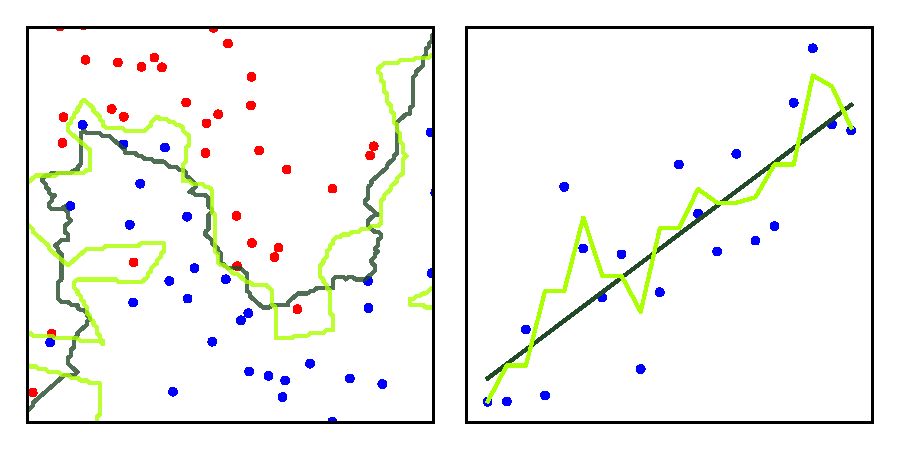
\includegraphics[width=12cm]{fig/lec08/bias_variance.pdf}
		\caption{Left: Decision boundaries in binary classification, $k$-nearest neighbors with one (bright) and nine (dark) neighbors. Right: Regression example, least squares (dark) and $2$-nearest neighbors (bright).}
		\label{fig:bias_variance}
	\end{figure}
}

\frame{\frametitle{Generalization error}
	
	\begin{block}{Supervised learning performance}
		SL performance is measured by a model's \hl{generalization error}, i.e., goodness of fit on unseen data.
	\end{block}\pause
	
	A data set is often finite as opposed to RL environments generating arbitrarily many observations.
	
	\begin{itemize}
	\item How to generate unseen data?\pause
	\begin{itemize}
		\item Hold out portions of the data set for \hl{cross-validation}.
	\end{itemize}
	\end{itemize}
	
}

\frame{\frametitle{$k$-fold cross-validation}
	\begin{columns}[t,onlytextwidth]
	\begin{column}{0.55\textwidth}
	\begin{minipage}[c]{\linewidth}
	
		\begin{figure}
			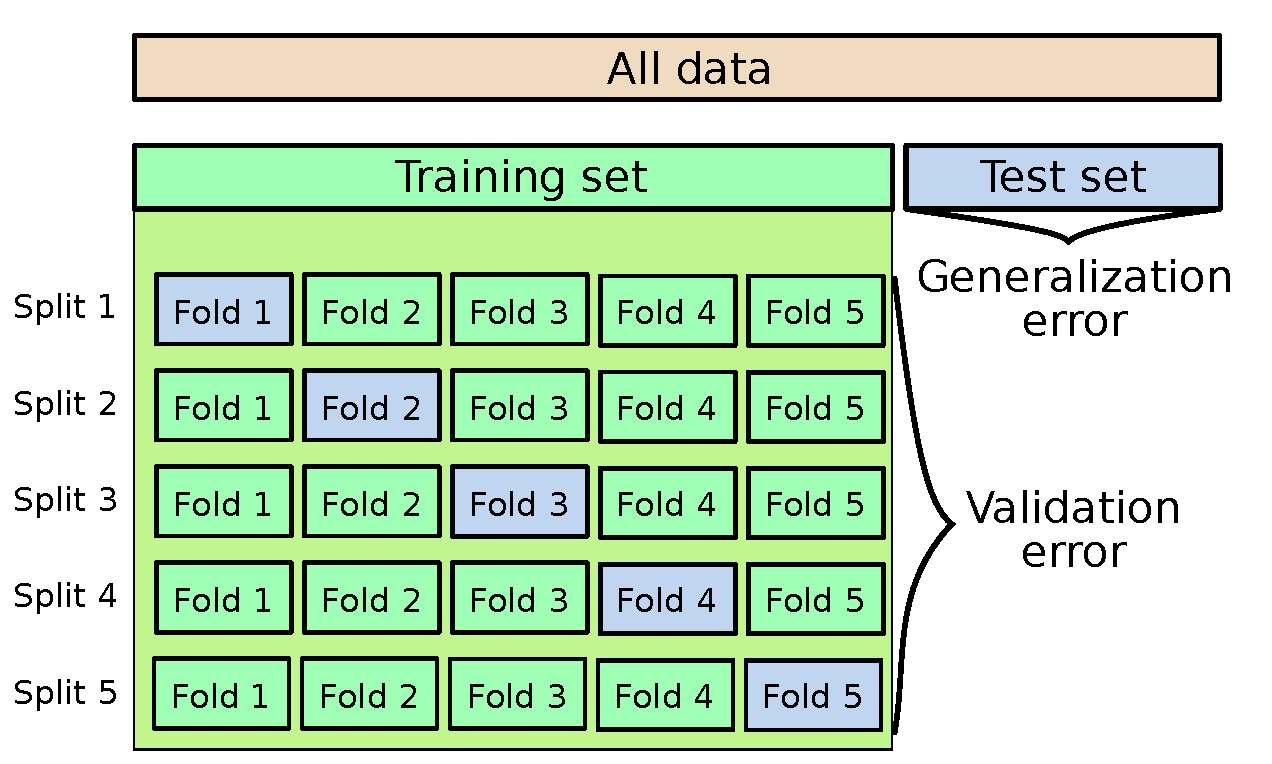
\includegraphics[width=\textwidth]{fig/lec08/kfold-cv.pdf}
			\caption{$k$-fold CV with five folds}
			\label{fig:kfold-cv}
		\end{figure}
	\end{minipage}
	\end{column}
	\hfill
	\begin{column}{0.45\textwidth}
	\begin{minipage}[c]{\linewidth}
		\begin{itemize}
		\item Cross-validation (CV) can be conducted with $k$-fold CV.\pause
		\item Training is repeated $k$ times with $k$ different splits of the training set.\pause
		\item Each observation serves as unseen instance at least once.\pause
		\item The validation error is an indicator for tuning hyperparameters.
		\end{itemize}
	\end{minipage}
	\end{column}
	\end{columns}
}


\frame{\frametitle{Means to improve an SL model}
	SL performance can be improved by:
	\begin{itemize}
		\item Collecting more data, i.e., increasing $K$ (more data is always better).\pause
		\item Choosing a more appropriate model.\pause
		\item Optimizing hyperparameters of the model.\pause
		\item Averaging over several different models (ensembling).\pause
		\item Most effectively: Revealing the most predictive patterns in the data to the model (feature engineering).
	\end{itemize}
}

%%%%%%%%%%%%%%%%%%%%%%%%%%%%%%%%%%%%%%%%%%%%%%%%%%%%%%%%%%%%%%%%%%
\subsection{Feature engineering}
%%%%%%%%%%%%%%%%%%%%%%%%%%%%%%%%%%%%%%%%%%%%%%%%%%%%%%%%%%%%%%%%%%

\frame{\frametitle{Feature engineering}
	Additional features might be:
	\begin{itemize}
		\item Coming from the real world via additional sensors or additional tracking mechanisms (think of a user's click behavior on a website)\pause
		\item Hand-designed (\textit{engineered}) by experts in the corresponding domain from the original feature set\pause
		\item Automatically built according to properties of each feature in the original set (Auto-ML)\pause
	\end{itemize}
	\begin{block}{Caution}
		Adding more features is not equivalent to having more data (which is always better).
		Having a fixed data set size, adding arbitrarily many features, regardless of their origin, increases chances to align statistical fluctuations with the target $\bm y_k$ - overfitting is the result.
	\end{block}
}

\frame{\frametitle{Feature engineering example (classification)}

	\begin{figure}
		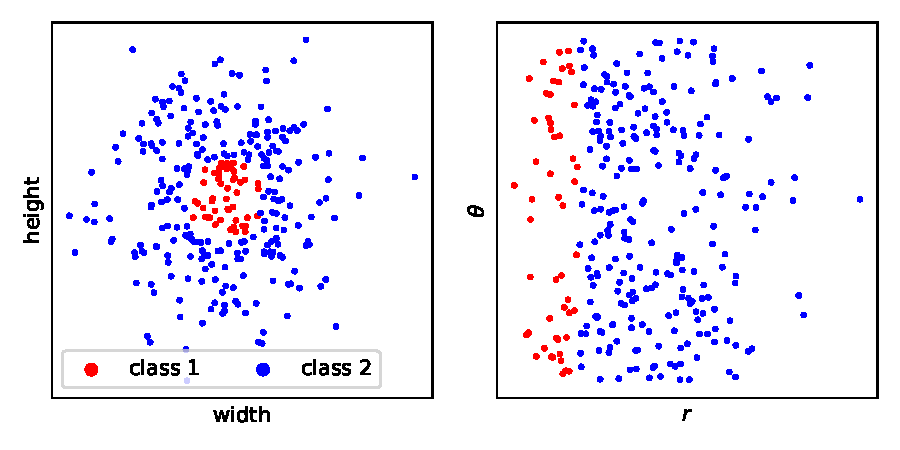
\includegraphics[width=11cm]{fig/lec08/fe_example.pdf}
		\caption{Features $r=\sqrt{\text{width}^2 + \text{height}^2}$ and $\theta = \arctan{(\frac{\text{height}}{\text{width}})}$ reveal linearly separable class distribution}
		\label{fig:fe_example}
	\end{figure}
	
}


\frame{\frametitle{Feature engineering example (regression)}
	\begin{figure}
		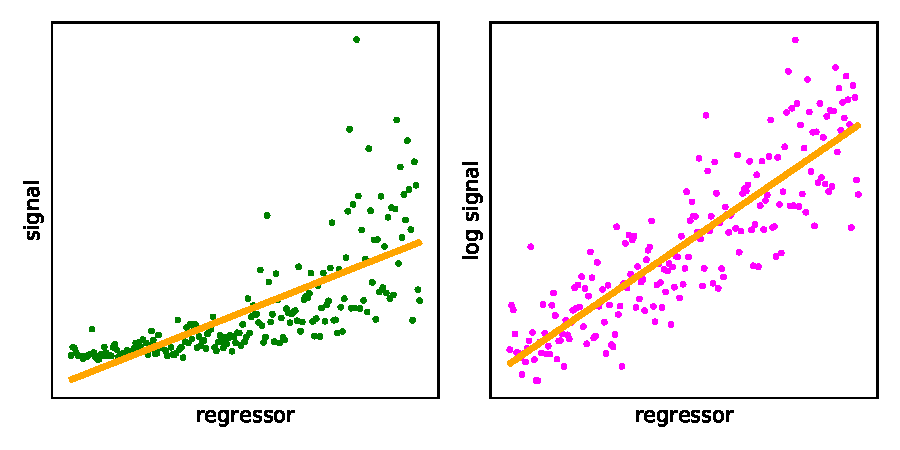
\includegraphics[width=11cm]{fig/lec08/fe_example2.pdf}
		\caption{Log-transform of the target signal exhibits linear relationship to the regressor}
		\label{fig:fe_example2}
	\end{figure}
}


\frame{\frametitle{Normalization}
Most models require data to be \hl{normalized} before training (apart from tree-based models).

Typical normalizaton schemes:
\begin{itemize}
	\item Standard scaling: $\tilde{ \bm x} = (\bm x- \text{Avg}(\bm x)) / \text{Std}(\bm x)$
	\item Min-Max scaling: $\tilde{\bm x} = (\bm x - \text{min}(\bm x))/ (\text{max}(\bm x) - \text{min}(\bm x))$
	\item Plain scaling: $\tilde{\bm x} = \bm x / \text{max}(| \bm x |)$
\end{itemize}

In an unnormalized data set, features with high variance will eclipse patterns in other features.
}

\frame{\frametitle{Data types}
Several different data types can be utilized for ML:
\begin{itemize}
	\item Binary: 1 or 0 (True or False).\pause
	\item Integer: $\mathbb{N}$ (e.g., number of rooms in a building).\pause
	\item Real-valued: $\mathbb{R}$ (e.g., temperature).\pause
	\item Categorical: like \{blue, green, red\}\pause
	\item Ordinal: Categoricals that can be ordered, e.g., educational experience (From elementary school to Ph.D.)
\end{itemize}

}

\frame{\frametitle{Data type specific normalization}

How to normalize categorical data?\pause

\begin{itemize}
	\item \textit{One-hot} encoding
		\begin{itemize}
			\item Replace a categorical of $n$ values with $n$ binary features.
			\item Feature space gets sparse and might get too big for memory. 
		\end{itemize}\pause
	\item Mean target encoding
	\begin{itemize}
		\item Replace each value of a categorical with the average (regression) or mode (classification) of the dependent variable being observed with the corresponding value.
		\item This might lead to information \textit{leaking} from the dependent variables into the independent variables, and might exhibit high performance that cannot be reproduced on unseen data.
	\end{itemize}\pause
	\item Entity embeddings
	\begin{itemize}
		\item Let a neural network find a cardinality-constrained set of real-valued features for each categorical.
		\item Works well in practice but is more intricate than alternatives.
	\end{itemize}
	
\end{itemize}
}

\frame{\frametitle{Typical feature engineering schemes}
	Feature design is often of the following form (tricks of the trade):
	
	Given $K$ feature vectors $\bm x_k \in \mathbb R^P$ with, e.g., $P=3$ (two real-valued regressors and a categorical independent variable $\bm x_k = (x_{k,r_1}, x_{k,r_2}, x_{k,c})$):\pause
	\begin{itemize}
		\item $\tilde x_{k} = x_{k,r_1} + x_{k,r_2}$ (or any other combination, e.g., product, division, subtraction, also cf. \figref{fig:fe_example}),\pause
		\item $\tilde x_k = x_{k,r} - \frac{1}{|\mathcal B|}\sum_{i \in \mathcal B} x_{i,r}\quad\forall r = \{r_1, r_2\}$ with $\mathcal B = \{i: x_{i,c} = x_{k, c}\}$,\pause
		\item Clip/drop/aggregate outliers away,\pause
		\item Coordinate transformations for spatial features (e.g., rotation),\pause
		\item In time domain:
		\begin{itemize}
			\item $\tilde{\bm{x}}_k = (x_{k,r_1}, x_{k-1,r_1}, x_{k-2,r_1}, x_{k,r_2}, x_{k,c})$ (lag features),
			\item $\tilde x_k = (1-\alpha)\tilde x_{k-1} + \alpha x_{k,r}$ (moving averages).
		\end{itemize}\pause
		\item In frequency domain:
		\begin{itemize}
			\item Amplitude and index of frequencies from a fast fourier transform (FFT)
		\end{itemize}
		
	\end{itemize}
}
%%%%%%%%%%%%%%%%%%%%%%%%%%%%%%%%%%%%%%%%%%%%%%%%%%%%%%%%%%%%%%%%%%
\subsection{Typical machine learning models}
%%%%%%%%%%%%%%%%%%%%%%%%%%%%%%%%%%%%%%%%%%%%%%%%%%%%%%%%%%%%%%%%%%

%  Model zoo (and their Hyperparameters)
\frame{\frametitle{Model landscape}
	When trying to find an appropriate mapping between input and output data, one can choose from a variety of models:\pause
	
	\begin{itemize}
		\item Linear/logistic regression (with regularization)
		\begin{itemize}
			\item The simplest data-fitting algorithm
		\end{itemize}\pause
		\item Support vector machines (SVM)
		\begin{itemize}
			\item Most popular algorithm before 2012
		\end{itemize}\pause
		\item (Deep) neural networks (DNN)
		\begin{itemize}
			\item Also coined as \textit{deep learning}, soared in popularity since 2012
			\item Most prevalent in the domains of natural language processing (NLP) and image processing
		\end{itemize}\pause
		\item Gradient Boosting Machines (GBM)
		\begin{itemize}
			\item Chaining of \textit{weak} models (most of the time decision trees)
			\item The best performing stand-alone model in tabular ML competitions
		\end{itemize}
	\end{itemize}
}

\frame{\frametitle{Model choice}
	\begin{figure}
		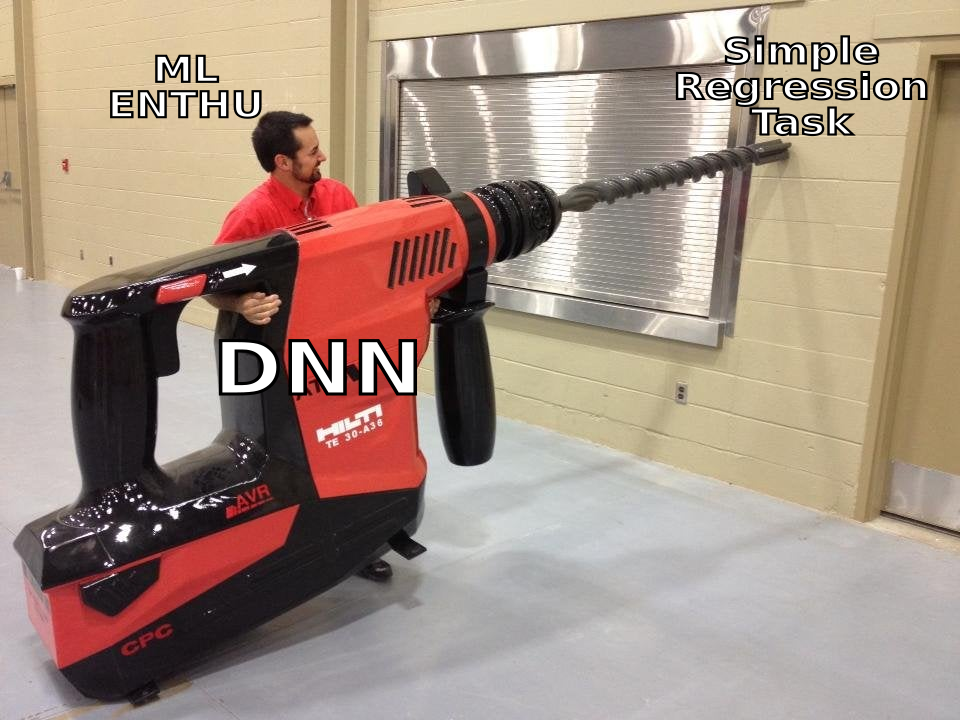
\includegraphics[width=8.8cm]{fig/lec08/bigdrill.png}
		\caption{Choose models appropriate for the problem! (Source: Adapted from \href{https://www.reddit.com/r/toolporn/comments/1kw63x/hilti_30c_in_your_hands_feels_huge_1050_x_750/}{reddit})}
		\label{fig:bigdrill}
	\end{figure}
}

%%%%%%%%%%%%%%%%%%%%%%%%%%%%%%%%%%%%%%%%%%%%%%%%%%%%%%%%%%%%%%%%%%
\subsection{Linear regression}
%%%%%%%%%%%%%%%%%%%%%%%%%%%%%%%%%%%%%%%%%%%%%%%%%%%%%%%%%%%%%%%%%%

\frame{\frametitle{Linear regression (1)}
Linear models assume a linear relationship between $\bm x_k = (1, x_{k,1}, x_{k,2},\dots,x_{k,P})$ and $y_k$ via trainable coefficients $\bm w \in \mathbb{R}^{P+1}$:
\begin{align}
	f(\bm x_k) &= \hat y_k = w_0 + \sum_{p=1}^P x_{k,p}w_p, \\
	\hat{\bm y}&= \bm{\Xi}\bm w,
\end{align}
where $\bm{\Xi} = (\bm x_1, \dots, \bm x_K)$. \pause
Among other methods, $\bm w$ can be estimated from $K$ samples by minimizing the residual sum of squares (RSS), which is coined the \hl{least squares} method:
\begin{equation}
	\text{RSS}(\bm w) = \sum_{k=1}^K (y_k - f(\bm x_k))^2 = (\bm y-\bm{\Xi w})\T(\bm y - \bm{\Xi w}).
	\label{eq:rss}
\end{equation}
}

\frame{\frametitle{Linear regression (2)}
	Deriving (\ref{eq:rss}) with respect to $\bm w$ and setting it to zero while assuming $\bm{\Xi}\T\bm{\Xi}$ is positive-definite, yields an analytically closed solution form:
	\begin{equation}
		\hat{\bm{y}} = \bm{\Xi\hat{w}} = \bm{\Xi} (\bm{\Xi}\T\bm{\Xi})^{-1}\bm{\Xi}\T\bm{y}.
		\label{eq:OLS_estimate}
	\end{equation}\pause
	
	\begin{alertblock}{Multicollinearity}
		If two regressors exhibit strong linear correlation, their coefficients can grow indeterministically.
		This corresponds to high variance in $\hat{\bm w}$.
		Regularization of $\hat{\bm w}$ alleviates this effect - it induces bias for less variance.
		Most prevalent linear regularized techniques are LASSO and Ridge:
		\begin{align}
			\text{RSS}_\text{LASSO}(\bm w) &= (\bm y-\bm{\Xi w})\T(\bm y - \bm{\Xi w}) + \lambda||\bm w||_1, \\
			\text{RSS}_\text{Ridge}(\bm w) &= (\bm y-\bm{\Xi w})\T(\bm y - \bm{\Xi w}) + \lambda||\bm w||_2,
			\label{eq:ridge}
		\end{align}
		where $\lambda$ controls the growth penalty.
	\end{alertblock}
}

%%%%%%%%%%%%%%%%%%%%%%%%%%%%%%%%%%%%%%%%%%%%%%%%%%%%%%%%%%%%%%%%%%
\subsection{Artificial neural networks}
%%%%%%%%%%%%%%%%%%%%%%%%%%%%%%%%%%%%%%%%%%%%%%%%%%%%%%%%%%%%%%%%%%

\frame{\frametitle{Artificial neural networks}
	Artificial neural networks (ANNs) describe nonlinear approximators $\hat{\bm y} = f(\bm{\Xi; \bm w})$ that are end-to-end differentiable.\pause
	\newline
	\begin{columns}[t,onlytextwidth]
	\begin{column}{0.45\textwidth}
	\begin{minipage}[c]{\linewidth}
	
		\begin{figure}
			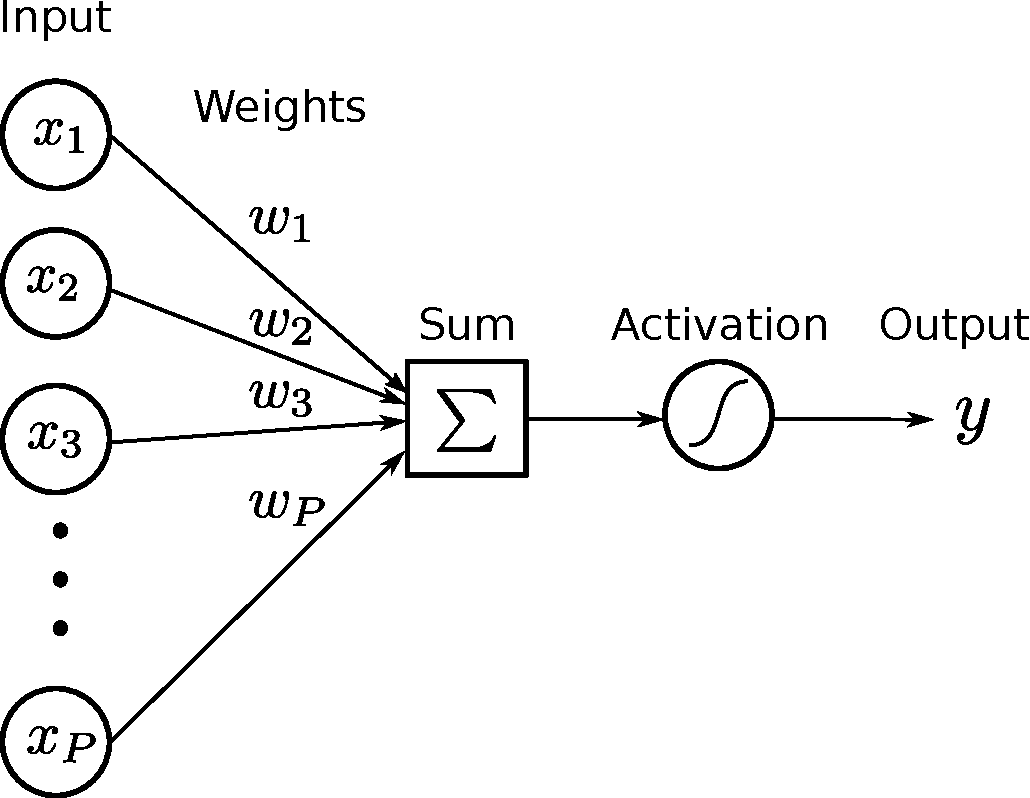
\includegraphics[width=0.9\textwidth]{fig/lec08/neuron.pdf}
			\caption{A typical neuron as the key building block of ANNs.}
			\label{fig:neuron}
		\end{figure}
	\end{minipage}
	\end{column}
	\hfill
	\begin{column}{0.55\textwidth}
	\begin{minipage}[c]{\linewidth}
		\begin{itemize}
		\item An ANN consists of \hl{nodes} or \hl{neurons} in one or more \hl{layers}.\pause
		\item Each node transforms the weighted sum of all previous nodes through an activation function.\pause
		\item The weighted connections are called \hl{edges}, which represent the ANN's parameters.
		\end{itemize}
	\end{minipage}
	\end{column}
	\end{columns}
	
}

\frame{\frametitle{Multi-layer perceptron}
	A vanilla ANN is the so-called \hl{feed-forward ANN} or \hl{multi-layer perceptron}.
	\newline
	\begin{columns}[t,onlytextwidth]
	\begin{column}{0.45\textwidth}
	\begin{minipage}[c]{\linewidth}
	
		\begin{figure}
			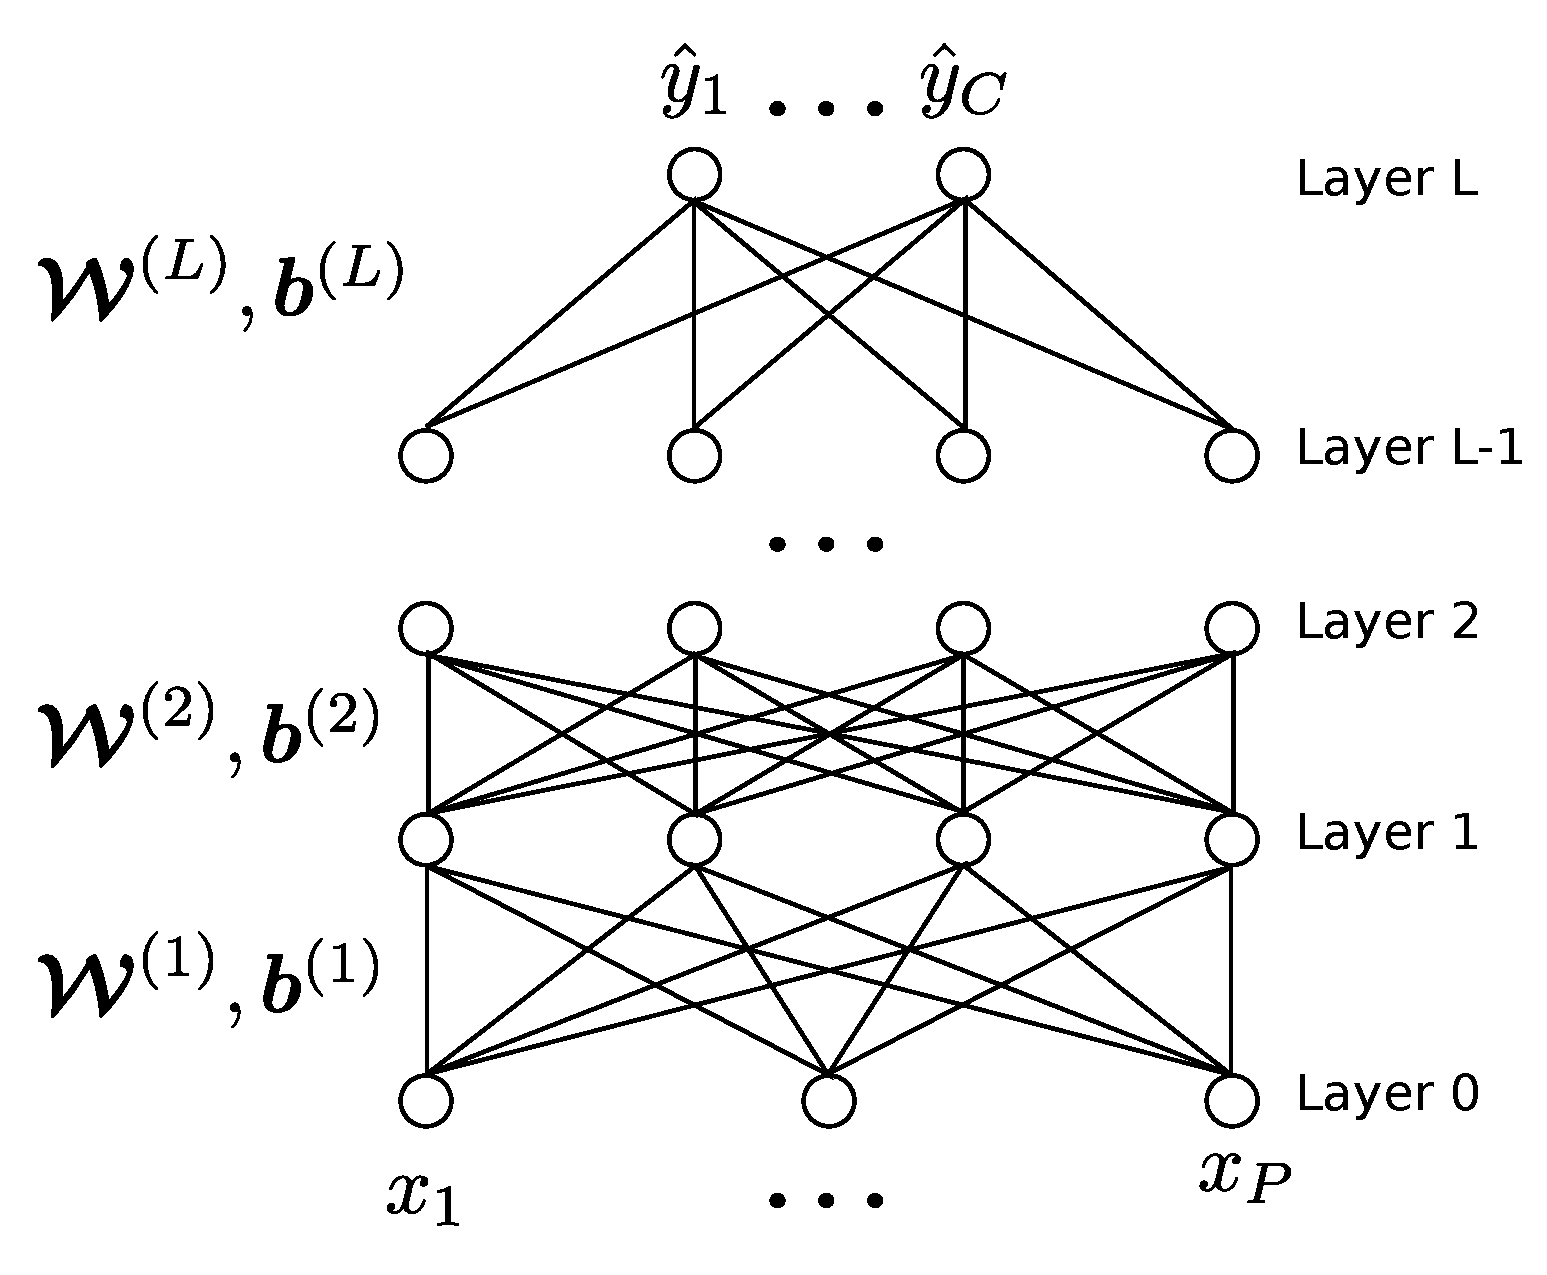
\includegraphics[width=0.8\textwidth]{fig/lec08/MLP.pdf}
			\caption{Multi-layer perceptron.}
			\label{fig:mlp}
		\end{figure}
	\end{minipage}
	\end{column}
	\hfill
	\begin{column}{0.5\textwidth}
	\begin{minipage}[r]{\linewidth}
		\begin{itemize}
		\item Only forward-flowing edges.\pause
		\item The \hl{depth} $L$ and width $H^{(l)}$ are hyperparameters.\pause
		\end{itemize}
		With $\varphi^{(l)}$ and $\bm{\mathcal Z}^{(l)}$ denoting the activation function and activation of layer $l$ respectively, we get for the output matrix $\bm{\mathcal H}^{(l)}$
		\begin{equation*}
			\bm{\mathcal H}^{(l)} = \varphi^{(l)}\big( \underbrace{\bm{\mathcal H}^{(l-1)}\bm{\mathcal{W}}^{(l)}  + \bm{b}^{(l)}}_{\bm{\mathcal Z}^{(l)}} \big).
		\end{equation*}
		
	\end{minipage}
	\end{column}
	\end{columns}\pause
	Weight matrix $\bm{\mathcal{W}}^{(l)} \in \mathbb{R}^{H^{(l-1)}\times H^{(l)}}$ and (broadcasted) bias matrix $\bm{b}^{(l)} \in \mathbb{R}^{K\times H^{(l)}}$ are iteratively optimized and denote the full set of parameters $\bm w$.
}

\frame{\frametitle{Activation functions}
	
	
	\begin{columns}[t,onlytextwidth]
	\begin{column}{0.45\textwidth}
	\begin{minipage}[c]{\linewidth}
		Within hidden layers most \\prevalent activation functions $\varphi(\cdot)$ are
		\begin{itemize}
			\item $h = \text{tanh}(z)$
			\item $h = \frac{1}{1+e^{-z}}$ (sigmoid)
			\item $h = \text{max}(0,z)$ \\(rectified linear unit (ReLU))
		\end{itemize}
		
	\end{minipage}
	\end{column}
	\hfill
	\begin{column}{0.52\textwidth}
	\begin{minipage}[r]{\linewidth}
		\begin{figure}
			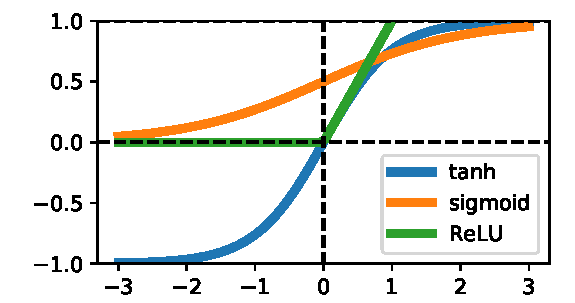
\includegraphics[width=0.8\textwidth]{fig/lec08/act_funcs.pdf}
			\caption{Common activation functions}
			\label{fig:act_funcs}
		\end{figure}
		
	\end{minipage}
	\end{column}
	\end{columns}\pause
	Whereas $\varphi^{(L)}(\cdot)$ is task-dependent:
		\begin{itemize}
			\item Regression: $\hat{{y}} = {h}^{(L)} = {z}^{(L)}$
			\item Binary classification: sigmoid
			\item Multi-class classification: 
			\begin{equation*}
			h_c^{(L)} = \frac{e^{z_c}}{\sum_{i=1}^C e^{z_i}}\quad\text{(softmax)}
			\end{equation*}
		\end{itemize}
}

\frame{\frametitle{Training neural networks (1)}
	ANN parameters are usually iteratively optimized via a variant of \hl{gradient descent}, e.g., stochastic gradient descent (SGD).
	\begin{align}
	\label{eq:weight_update}
		\bm{\mathcal{W}}^{(l)} &\leftarrow \bm{\mathcal{W}}^{(l)} - \alpha \nabla_{\bm{\mathcal{W}}^{(l)}} \mathcal{L}(\bm y, \hat{\bm y}),\\
		\label{eq:bias_update}
		\bm{b}^{(l)} &\leftarrow \bm{b}^{(l)} - \alpha \nabla_{\bm{b}^{(l)}} \mathcal{L}(\bm y, \hat{\bm y}),
	\end{align}
	with $\alpha$ being the step size and $\mathcal{L}(\cdot)$ denoting the \hl{loss} between the ground truth vector and the estimation vector.\pause
	
	
Typical loss functions:

\begin{itemize}
	\item Regression: (root) mean squared error (RMSE), mean absolute error
	\item Classification: Cross-entropy (CE)
\end{itemize}
Several iterations over the data set $\bm{\mathcal D}$ are called \hl{epochs}.
}

\frame{\frametitle{Training neural networks (2)}
\begin{columns}[t,onlytextwidth]
	\begin{column}{0.45\textwidth}
	\begin{minipage}[c]{\linewidth}
		\begin{figure}
		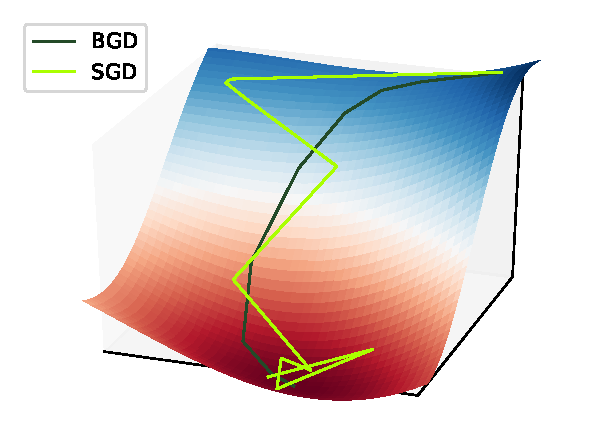
\includegraphics[width=0.8\textwidth]{fig/lec08/sgd.pdf}
		\caption{BGD vs. SGD}
		\label{fig:sgd}
	\end{figure}
	\end{minipage}
	\end{column}
	\hfill
	\begin{column}{0.52\textwidth}
	\begin{minipage}[r]{\linewidth}
		Gradient descent alternatives:
		\begin{itemize}
			\item Batch gradient descent (BGD): Average gradients over all samples, then update weights.
			\item Stochastic gradient descent (SGD): Update weights after each sample.
		\end{itemize}
			
	\end{minipage}
	\end{column}
	\end{columns}
	SGD is more computationally  efficient, but steps are more random.
	
	Nowadays, mini-batch gradient descent (mix of SGD and BGD) and further improvements are used, e.g., momentum and second derivatives, to ensure faster convergence to better optima.
}



\frame{\frametitle{Training neural networks (3)}
	\textbf{How to retrieve the gradients:}
	
	Recall chain rule for vector derivatives, e.g., with $\bm y = g(\bm x)$ and $z = f(\bm y)$ where $g: \mathbb{R}^m \rightarrow \mathbb{R}^n$ and $f: \mathbb{R}^n \rightarrow \mathbb{R}$:
	\begin{equation}
		\nabla_{\bm x}z = \frac{\partial z}{\partial \bm x} = {\underbrace{\bigg( \frac{\partial \bm y}{\partial \bm x}\bigg)}_{\text{Jacobian of g }}}\T\cdot \underbrace{\frac{\partial z}{\partial\bm y}}_\text{gradient} = \sum_{j} \frac{\partial y_j}{\partial \bm x}\cdot\frac{\partial z}{\partial y_j}.
	\end{equation}\pause
	This can be used equivalently for matrices/tensors of any shape $\nabla_{\bm{\Xi}}y = \frac{\partial y}{\partial \bm{\Xi}}$ when we assume to enumerate each element of the tensor consecutively and loop through them.\pause
	
	\begin{block}{Error Backpropagation}
		After a \hl{forward step} through the network, make a \hl{backward step} in which the gradient $\bm\gamma$ of the loss $\mathcal{L}(\bm y, \hat{\bm y})$ is computed w.r.t the ANN's parameters from the output layer back to the input layer.
	\end{block}
}

\frame{\frametitle{Training neural networks (4)}
	\setlength{\algomargin}{0.5em}
	\begin{algorithm}[H]
	\SetKwInput{Input}{input} 
	\SetKwInput{Output}{output}
	\SetKwInput{Init}{init}
	\SetKwInput{Param}{parameter}
	\Init{$\bm{\mathcal H}^{(0)} \leftarrow \bm{\Xi}$}
	// forward propagation\\
	\For{$l=1,\ldots,L$ layers}{ 
		$\bm{\mathcal Z}^{(l)} \leftarrow \bm{\mathcal H}^{(l-1)}\bm{\mathcal{W}}^{(l)} + \bm{b}^{(l)}$\\
		$\bm{\mathcal H}^{(l)} \leftarrow \varphi^{(l)}(\bm{\mathcal Z}^{(l)})$\\
	}
	// backward propagation\\
	$\bm\gamma \leftarrow \nabla_{\bm{h}^{(L)}}\mathcal{L}(\bm y, \hat{\bm y})$ // note that $\bm{h}^{(L)} = \hat{\bm y}$\\
	\For{$l= L, \ldots, 1$ layers}{
		$\bm\gamma \leftarrow \bm\gamma \odot \partial (\varphi^{(l)})(\bm{\mathcal Z}^{(l)}) = \nabla_{\bm{\mathcal Z}^{(l)}} \mathcal{L}(\bm y, \hat{\bm y})$ // $\odot$: elementwise mult.\\
		Append $\bm\gamma = \nabla_{\bm{b}^{(l)}} \mathcal{L}(\bm y, \hat{\bm y})$ to list of bias gradients\\
		Append $(\bm{\mathcal H}^{(l-1)})\T\cdot\bm\gamma  = \nabla_{\bm{\mathcal W}^{(l)}} \mathcal{L}(\bm y, \hat{\bm y})$ to list of weight gradients\\
		$\bm\gamma \leftarrow \bm\gamma\cdot(\bm{\mathcal W}^{(l)})\T = \nabla_{\bm{\mathcal H}^{(l-1)}}\mathcal{L}(\bm y, \hat{\bm y})$\\
	}
		
	\caption{Error backpropagation}
	\label{algo:errorbp}
	\end{algorithm}
}

\frame{\frametitle{Error backpropagation example (1)}
Assume $\bm x_0 = [2, 5, 7], y_0 = 2.5$, and a two-layered ANN with the MSE cost, and sigmoid activation functions $\sigma(z) = \frac{1}{1+e^{-z}}$.
The hidden layer contains two neurons with output $\bm h^{(1)} \in \mathbb{R}^2$, while the weight vectors are initialized with $\bm{\mathcal W}^{(1)} = \big[\begin{smallmatrix} 0.1& -0.3 & 0.2\\
												0.0& 0.4 & -0.9 \\\end{smallmatrix} \big]\T, \bm b^{(1)} = [0.05, -0.03]$,  and $\bm{\mathcal W}^{(2)} = [ 0.2, -0.8]\T, \bm b^{(2)} = [0.1]$.\pause
			
Applying SGD, we start with forward propagation:
\begin{align*}
	\bm h^{(1)} &= \varphi^{(1)}(\bm{x}_0\bm{\mathcal{W}}^{(1)} + \bm{b}^{(1)}) \\
	\quad &= \sigma([0.1, -4.3] + [0.05, -0.03]) = [0.53, 0.01]\\
	\hat{y}_0 &= \bm{h}^{(1)}\bm{\mathcal{W}}^{(2)} + \bm{b}^{(2)} = 0.198
\end{align*}
				
}

\frame{\frametitle{Error backpropagation example (2)}
	Backpropagation (with $\sigma^\prime(z) = \partial_z \sigma(z) = \sigma(z)(1-\sigma(z))$):
	
	\begin{align*}
		\bm\gamma^{(2)} = \nabla_{\hat{y}_0}\mathcal{L}(y_0, \hat{y_0}) &= \nabla_{\hat{\bm{y}}} (y_0 - \hat y_0)^2 = -2 (y_0 - \hat y_0) = -4.604\\
		\nabla_{\bm{b}^{(2)}} \mathcal{L}(y_0, \hat{y_0}) &= \bm\gamma^{(2)} \odot \partial (\varphi^{(2)})(\bm z^{(2)}) = \bm\gamma^{(2)} \\
		\nabla_{\bm{\mathcal W}^{(2)}} \mathcal{L}(y_0, \hat{y}_0) &= (\bm{h}^{(1)})\T\cdot\bm\gamma^{(2)} = [-2.44, -0.046]\T\\
		\bm\gamma^{(1)} = \nabla_{\bm{h}^{(1)}}\mathcal{L}(y_0, \hat{y}_0)&= \bm\gamma^{(2)}\cdot(\bm{\mathcal W}^{(2)})\T = [-0.921, 3.683]\\
		\nabla_{\bm{b}^{(1)}} \mathcal{L}(y_0, \hat{y_0}) &= \bm\gamma^{(1)} \odot \partial (\varphi^{(1)})(\bm z^{(1)}) = \bm\gamma^{(1)}\odot \sigma^\prime(\bm{x}_0\bm{\mathcal{W}}^{(1)} + \bm{b}^{(1)}) \\
		\quad &= \bm\gamma^{(1)}\odot (\bm h^{(1)}(1-\bm h^{(1)})) = [-0.229, 0.036]\\
		\nabla_{\bm{\mathcal W}^{(1)}} \mathcal{L}(y_0, \hat{y}_0) &= \bm{x}_0\T\cdot\bm\gamma^{(1)} = \big[\begin{smallmatrix} -1.84 & -4.605 & -6.447\\ 7.366& 18.415 & 25.781 \\\end{smallmatrix} \big]\T
	\end{align*}
	
	Now update weights and biases according to (\ref{eq:weight_update}) and (\ref{eq:bias_update}).
}




\frame{\frametitle{Weight initialization}

Early in deep learning research, it was found that random uniform or random normal weight initialization leads to poor training.

According to Glorot and Bengio\footnote[1]{X. Glorot and Y. Bengio, "Understanding the difficulty of training deep feedforward neural networks", \textit{Proceedings of Machine Learning Research}, 2010}, use the following layer-specific initialization schemes (with $H_\text{in}$ and $H_\text{out}$ denoting amount of hidden units of previous and current layer, respectively):
\begin{itemize}
	\item uniform: $\bm{w} \sim \mathcal{U}\Big(-\frac{\sqrt{6}}{\sqrt{H_\text{in}+H_\text{out}}}, \frac{\sqrt{6}}{\sqrt{H_\text{in}+H_\text{out}}} \Big)$
	\item normal: $\bm{w} \sim \mathcal{N}\Big(0, \frac{\sqrt{2}}{\sqrt{H_\text{in}+H_\text{out}}}  \Big)$
\end{itemize}\pause

Please note that generally due to the random weight initialization the result of repeated error backpropagation training is always different regardless of having the same hyperparameters and the same data.

This equals to \hl{local optimization in highly non-linear parameter spaces at random starting points}.
}

\frame{\frametitle{Regularizing neural networks}
	In order to mitigate overfitting, ANNs must be regularized by
	\begin{itemize}
		\item weight decay, i.e., adding an $\ell_2$ penalty term to the weights, see (\ref{eq:ridge}), \pause
		\item layer normalization during training,
		\begin{itemize}
			\item i.e all layers' activations are normalized by standard scaling separately,
		\end{itemize}\pause
		\item dropout, i.e., randomly disable nodes' contribution.
		\begin{itemize}
			\item This helps especially in deep networks,
			\item and effectively builds an ensemble of ANNs with shared edges.
		\end{itemize}
	\end{itemize}
}

\frame{\frametitle{Advanced topologies}
	\begin{figure}[tbp]
    \centering
    \begin{minipage}[t]{0.38\textwidth}
        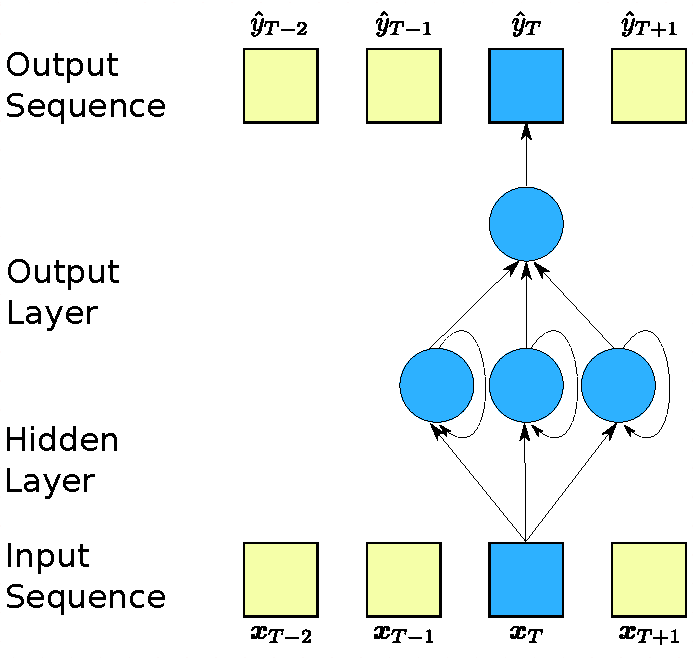
\includegraphics[width=\textwidth]{fig/lec08/RNN_over_sequence.pdf}
    \end{minipage}\hfill
    \begin{minipage}[t]{0.55\textwidth}
        \centering
        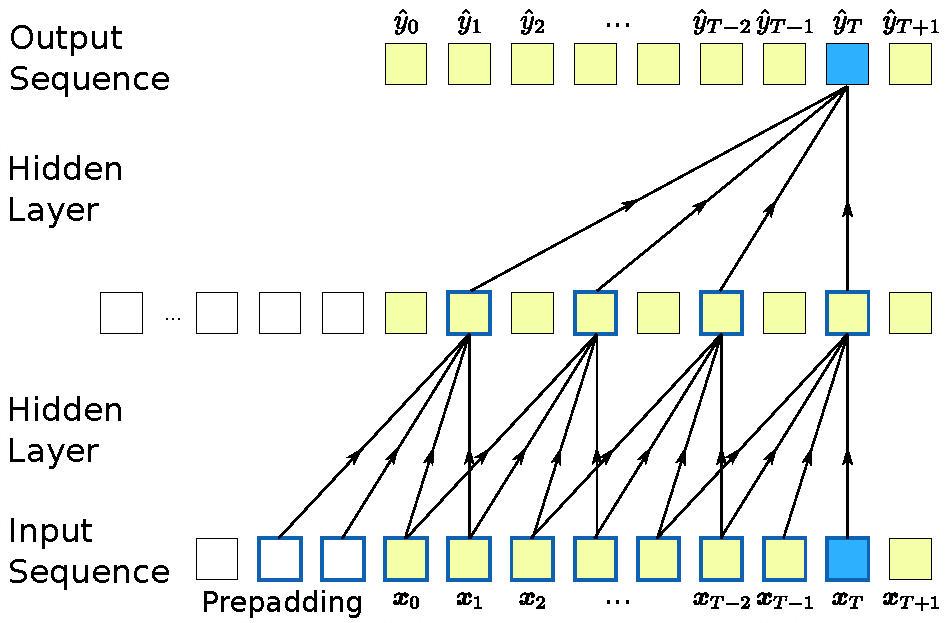
\includegraphics[width=\textwidth]{fig/lec08/CNN_over_sequence.pdf}
        \end{minipage}
        \caption{Recurrent (left) and 1-D convolutional (right) ANNs are more appropriate in time domains, e.g., where the given data set has a dynamic system background}
\end{figure}
}

\frame{\frametitle{Hyperparameter optimization (1)}
	\begin{figure}
		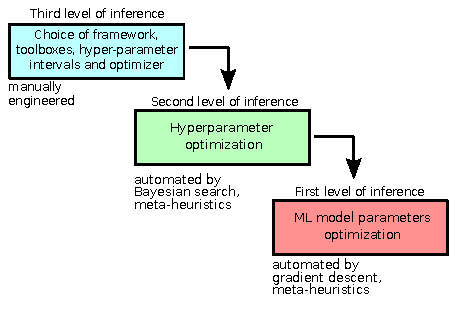
\includegraphics[width=9cm]{fig/lec08/levels_of_opt.pdf}
		\caption{The three levels of optimization}
		\label{fig:levels_of_opt}
	\end{figure}
	
}

\frame{\frametitle{Hyperparameter optimization (2)}
	\begin{itemize}
		\item Hyperparameter optimization is, again, a non-linear optimization problem.
		\item Evaluation of any point in this space can be very costly, though.
		\item Information gathered during a search must be fully utilized.
		\item Toolboxes (incomprehensive)
		\begin{itemize}
			\item \href{https://github.com/optuna/optuna}{Optuna}
			\item \href{https://scikit-optimize.github.io/stable/}{Scikit-optimize}
			\item \href{https://pyswarms.readthedocs.io/en/latest/}{Pyswarm}
		\end{itemize}
	\end{itemize}
}

\frame{\frametitle{SL toolboxes}
	\begin{itemize}
		\item Deep learning
		\begin{itemize}
			\item \href{https://www.tensorflow.org/tutorials/quickstart/beginner}{Tensorflow 2 (Keras)}
			\item \href{https://pytorch.org/}{PyTorch}
			\item \href{https://chainer.org/}{Chainer}
			\item \href{https://docs.microsoft.com/en-us/cognitive-toolkit/}{CNTK}
		\end{itemize}\pause
		\item Gradient boosting machines
		\begin{itemize}
			\item \href{https://xgboost.readthedocs.io/en/latest/}{XGBoost}
			\item \href{https://lightgbm.readthedocs.io/en/latest/}{LightGBM}
			\item \href{https://catboost.ai/}{CatBoost}
		\end{itemize}\pause
		\item Linear, tree-based, memory-based models, SVMs, among others
		\begin{itemize}
			\item \href{https://scikit-learn.org/stable/}{Scikit-learn}
		\end{itemize}
	\end{itemize}		

}


%%%%%%%%%%%%%%%%%%%%%%%%%%%%%%%%%%%%%%%%%%%%%%%%%%%%%%%%%%%%%
%% Summary %%
%%%%%%%%%%%%%%%%%%%%%%%%%%%%%%%%%%%%%%%%%%%%%%%%%%%%%%%%%%%%%
\begin{frame}
\frametitle{Summary: what you've learned today}
\begin{itemize}
	\item Industry has high demand for ML applications.\pause
	\item Higher bias trades off variance for a better overall score.\pause
	\item How to cross-validate and improve SL models.\pause
	\item How features are engineered and normalized.\pause
	\item Fundamentals of linear regression and neural networks.
\end{itemize}
\end{frame}
